% ============================================================================================================
\chapter{Backtest 2010-2025}\label{ch:backtest}
% ============================================================================================================

\section{Méthode : calibration et validation séparées}

\begin{itemize}
\item \textbf{Temps réel.} Pour une rétrosimulation partant de l'année $B$, les coefficients des équations sont estimés
sur des données allant jusqu'à $B$ seulement ; le PIB potentiel est reconstruit avec la productivité globale des
facteurs filtrée jusqu'à $B$ puis prolongée à son rythme des huit dernières années ; le chômage structurel est filtré
jusqu'à $B$ puis maintenu. Aucune information postérieure à l'origine n'entre dans les paramètres.
\item \textbf{Exogènes observées.} Comme dans toute évaluation conditionnelle, les variables que le modèle ne cherche pas
à expliquer sont celles observées ex post : demande et prix mondiaux, prix d'importation (dont l'énergie), consommation
publique, population active, taux longs, taux d'IS, prestations en volume, autres dépenses publiques, et les politiques
fiscales sous forme de taux apparents de recettes (impôts sur les produits, impôts des ménages, cotisations). Les
politiques sont des données, pas des résultats.
\item \textbf{Variables validées} (jamais injectées) : PIB, consommation, investissement, exportations, importations,
emploi, chômage, productivité, prix, salaire réel, recettes, dépenses, solde et dette publics.
\item \textbf{Origines.} 2010 (jusqu'en 2019 : crise de la zone euro, consolidation, CICE, reprise), 2012, 2014, 2016
(jusqu'en 2019), et 2021 (jusqu'en 2025 : choc énergétique et inflationniste, hausse des taux). La crise sanitaire
(2020-2021) n'a pas de mécanisme dans le modèle (confinements, activité partielle) : elle est exclue des simulations
continues plutôt que neutralisée artificiellement.
\item \textbf{Références.} Modèle naïf (croissance moyenne des cinq années précédant l'origine) ; modèle de demande
seul ; fermetures de la v0.6 et de la v0.7. Le modèle bénéficie des exogènes observées, que le modèle naïf n'utilise
pas : la comparaison mesure la valeur des mécanismes conditionnellement à ces exogènes, pas une capacité de
prévision.
\end{itemize}

\section{Résultats}

\begin{figure}[htbp]\centering
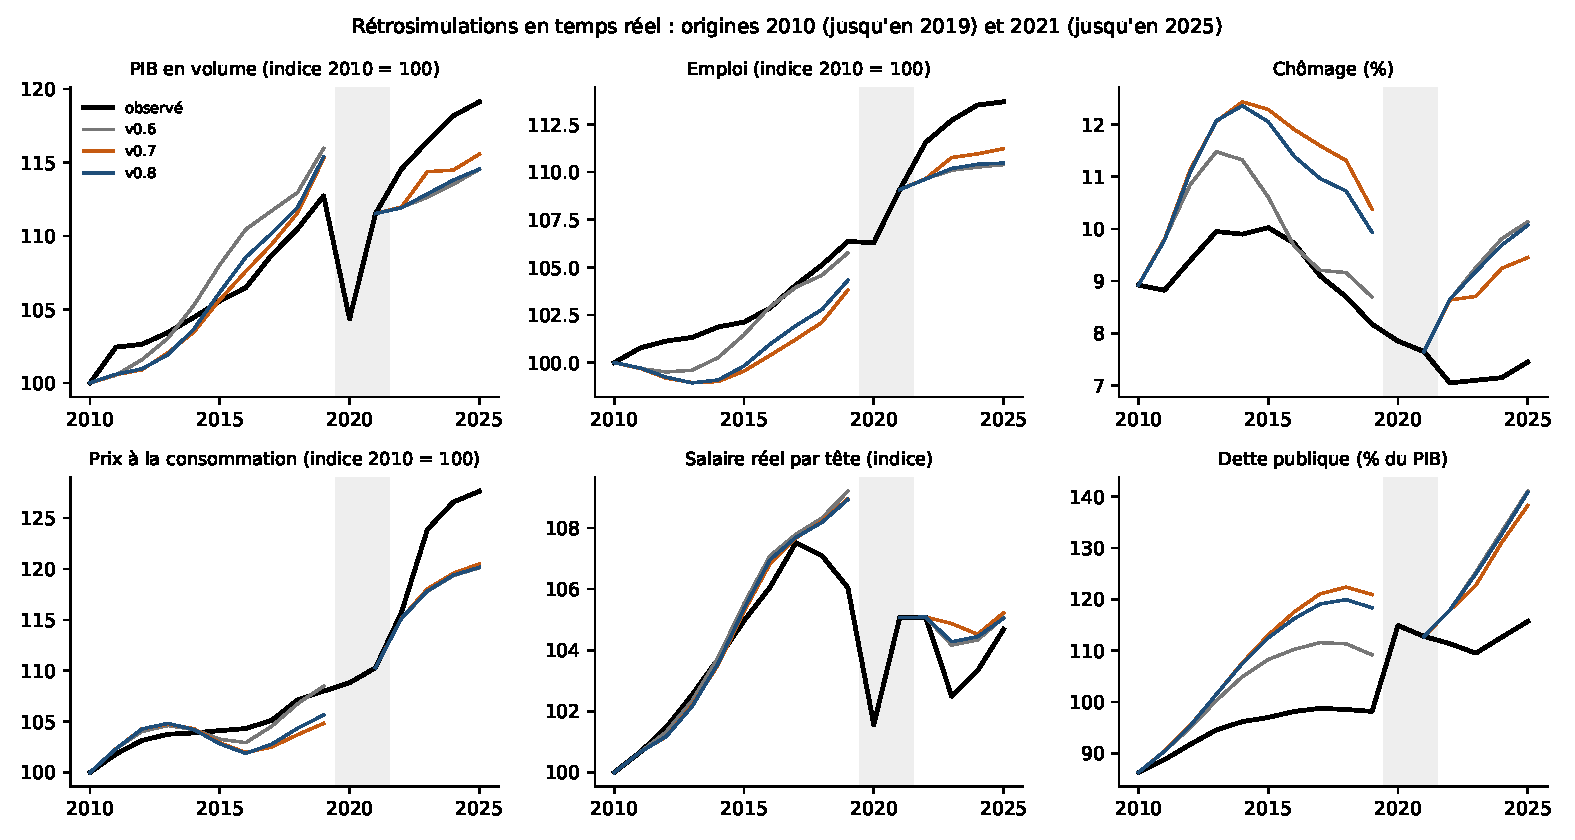
\includegraphics[width=\linewidth]{backtest.pdf}
\caption{Rétrosimulations en temps réel (noir : observé). La zone grise est la crise sanitaire, non simulée.}\label{fig:backtest}
\end{figure}

\begin{table}[htbp]\centering\scriptsize
\caption{Erreur quadratique moyenne des rétrosimulations : taux de croissance annuels (points) pour les volumes, les
prix et le salaire réel ; niveaux (points) pour le chômage et les ratios de finances publiques.}\label{tab:rmse}
\tabfit{../tables/backtest_rmse.tex}
\end{table}

\begin{table}[htbp]\centering\small
\caption{Erreur de niveau selon l'horizon (origine 2010, modèle v0.8).}\label{tab:horizons_bt}
\tabfit{../tables/backtest_horizons.tex}
\end{table}

\paragraph{Ce que le modèle reproduit raisonnablement.}
\begin{itemize}
\item \textbf{La croissance du PIB} : erreur de 0,5 à 1 point par an selon la période, l'erreur de niveau restant
inférieure à 2,5 \% après neuf ans (origine 2010). Le modèle ne fait mieux que le modèle naïf que sur deux
périodes sur cinq (2012-2019 et 2016-2019) ; il fait moins bien sur 2010-2019, 2014-2019 et 2021-2025, ce qui
rappelle qu'un modèle structurel n'est pas un outil de prévision de court terme.
\item \textbf{Les recettes publiques en part du PIB} : erreur de 0,3 à 0,9 point, une fois les taux apparents observés
fournis. Sans ces politiques, l'erreur atteint 2,8 points : la consolidation de 2011-2013 est d'abord fiscale.
\item \textbf{Les prix} sur 2010-2019 (0,6 à 0,8 point par an).
\end{itemize}

\paragraph{Ce qu'il reproduit mal.}
\begin{itemize}
\item \textbf{L'emploi et le chômage de 2010-2019} : le modèle sous-estime l'emploi de 2 \% en 2019 et surestime le
chômage de 1,8 point. Les créations d'emplois de 2015-2019, riches en emplois et pauvres en productivité, ne sont
pas reproduites : la productivité simulée croît trop (+4,4 \% d'erreur de niveau en 2019). Deux causes : le potentiel
« en temps réel » extrapole la tendance de productivité d'avant 2010, alors que la productivité française a ralenti ;
et les baisses du coût du travail (CICE, pacte de responsabilité), fournies en exogène dans une variante, passent
surtout dans les prix et peu dans l'emploi (variante « coût du travail » : le chômage n'est pas mieux reproduit).
\item \textbf{La dette} : +20 points d'erreur en 2019. Décomposition par bloc (tableau~\ref{tab:bloc}) : les recettes
sont reproduites ; les dépenses sont trop élevées de 1,4 à 2,6 points, du fait d'une charge d'intérêts trop lente à
baisser (taux apparent de 2,6 \% simulé contre 2,2 \% observé en 2015 : le renouvellement d'un huitième de la dette
par an est trop lent quand les taux chutent), de prestations plus élevées (chômage surestimé, stabilisateur) et d'un
PIB nominal plus bas. Erreur de structure (renouvellement de la dette) et de paramètre (productivité).
\item \textbf{Le choc de 2022-2023} : l'inflation est sous-estimée de 6 points en niveau en 2025 (l'énergie importée est
fournie, mais pas les boucliers tarifaires ni les effets de second tour sur les marges) et les exportations sont
surestimées de 8 \% (aéronautique, énergie, tourisme). Erreurs principalement de données et de structure.
\end{itemize}

\begin{table}[htbp]\centering\small
\caption{Test par bloc des finances publiques (origine 2010, modèle v0.8) : simulé / observé, en \% du PIB.}\label{tab:bloc}
\tabfit{../tables/backtest_bloc.tex}
\end{table}

\paragraph{Comparaison des fermetures.} Sur 2010-2019, la fermeture de la v0.8 fait mieux que celle de la v0.7 sur le
chômage (1,9 contre 2,2), la dette (15 contre 16) et les dépenses (1,8 contre 2,0), un peu moins bien sur le PIB
(1,0 contre 0,9) et la consommation ; elle fait mieux que le modèle de demande seul sur le chômage et la dette. Mais la fermeture de la v0.6, ancrée sur le chômage structurel
filtré, reproduit mieux le chômage (1,0) et la dette (9,7) : elle s'appuie directement sur le marché du travail,
alors que la fermeture sur le potentiel hérite de l'erreur de productivité en temps réel. Sur 2014-2019, 2016-2019 et
2021-2025, les écarts entre fermetures sont faibles. Les variantes de θ (0,5 et 1,0) ne se distinguent pas sur cette
période : le backtest ne permet pas de discriminer θ, ce qui justifie de le conserver comme incertitude.

\begin{resultat}[Bilan du backtest]
Le modèle est satisfaisant sur le PIB, les recettes et les prix hors choc énergétique ; médiocre sur l'emploi des
années 2015-2019, sur la charge d'intérêts quand les taux varient vite et sur le choc inflationniste de 2022. Les
erreurs sont surtout systématiques (biais de productivité, d'intérêts) plutôt que ponctuelles. La fermeture sur le
potentiel n'est pas validée comme meilleure que la fermeture sur le chômage sur 2010-2019 : elle est retenue pour sa
cohérence avec les chocs d'offre (document 15), pas pour sa performance historique.
\end{resultat}

\section{Reproduire les effets de politiques publiques}

\begin{table}[htbp]\centering\scriptsize
\caption{Effets simulés et évaluations empiriques (simulations v0.8, comportements centraux).}\label{tab:politiques}
\tabfit{../tables/politiques.tex}
\end{table}

La distinction entre évaluations causales (expériences naturelles, différences de différences, discontinuités) et
estimations par modèle est indiquée. Lecture :
\begin{itemize}
\item \textbf{Coût du travail} : $+132\,000$ emplois en 2030 et $+159\,000$ en 2032 pour une baisse de 20\md{} de
cotisations employeurs, entre l'évaluation microéconométrique du CICE (100 000) et les estimations par modèle (160 000).
La v0.8 ne s'éloigne pas de la v0.7 sur ce point.
\item \textbf{TVA} : $+0{,}36$ \% sur les prix après un an pour un point de hausse du taux normal (répercussion
d'environ 60 \% la première année), $-0{,}19$ \% pour une baisse. L'asymétrie est imposée par hypothèse, d'après
Benzarti et al. (2020) ; le niveau de la répercussion est dans la fourchette de Carbonnier (2007).
\item \textbf{IS} : $+0{,}85$ \% d'investissement des entreprises en 2032 pour une baisse du taux à 20 \%, soit une
élasticité au coût d'usage implicite dans le bas de la fourchette internationale ; aucune évaluation française causale
d'une baisse d'IS ne permet de trancher.
\item \textbf{Investissement public} : multiplicateur de 0,6 la première année comme la troisième, dans le bas de la
fourchette (le modèle n'intègre pas d'effet de l'investissement public sur la productivité, ce qui explique l'absence
de hausse à moyen terme).
\item \textbf{Assurance chômage} : la baisse de 25 \% des allocations augmente l'emploi structurel de 54 000 personnes
(environ $-0{,}16$ point de chômage structurel), mais l'effet de demande domine jusqu'en 2035 ($+0{,}10$ point de
chômage en 2030) et le chômage effectif ne baisse que de 0,08 point en 2047. La convergence est lente parce que l'emploi
s'ajuste progressivement à la production. L'effet de long terme est faible au regard des élasticités micro de la durée
du chômage ; il est cohérent avec les travaux qui trouvent des effets macroéconomiques plus faibles.
\item \textbf{Offre de travail} : $+107\,000$ actifs pour une hausse de 25 \% de la prime d'activité, $-72\,000$ pour
une hausse de 25 \% du RSA. Ces effets sont \emph{dans le haut} des évaluations françaises, qui trouvent des effets de
participation faibles (Bargain et Vicard 2014, au seuil d'éligibilité au RSA à 25 ans). Ils sont conservés en valeur
centrale parce qu'ils proviennent d'élasticités structurelles appliquées aux gains au travail calculés par OpenFisca,
mais la configuration « réactions faibles » (élasticités divisées par 2,5 environ) est au moins aussi plausible.
\end{itemize}
